The derivation follows the one-dimensional, small-motion model used in the course notes (pp. 103--105). The tube has rigid walls and constant cross-sectional area $A$. The fluid is inviscid, has uniform equilibrium density $\rho$, and has constant bulk modulus $K$. There is no mean flow. Subscripts $x$ and $t$ denote partial derivatives with respect to position and time. The pressure variable below is the acoustic pressure disturbance, so the total pressure is $P(x,t)=P_0+p(x,t)$, where the uniform equilibrium pressure $P_0$ has zero spatial gradient.

\textbf{1. Displacement and pressure disturbance.} Let $u(x,t)$ be the small axial displacement of a fluid particle whose equilibrium position is $x$. The associated pressure disturbance is $p(x,t)$. The element initially occupying $[x,x+d x]$ has left and right displacements $u(x,t)$ and $u(x+d x,t)$, respectively. A first-order Taylor expansion gives

\[
u(x+d x,t)=u(x,t)+u_x(x,t)d x,
\qquad
p(x+d x,t)=p(x,t)+p_x(x,t)d x.
\]

The longitudinal strain is therefore $u_x$. The symbol $p$ denotes the perturbation from equilibrium; the constant $P_0$ cancels from the force balance.

\textbf{2--3. Infinitesimal element and free-body diagram.} The element and its pressure forces are shown below. The two displacement arrows describe the particle motion at the element faces. The force arrows in the lower panel are pressure forces. Pressure on the left face acts in the positive $x$ direction, while pressure on the right face acts in the negative $x$ direction.

\begin{figure}[H]
\centering
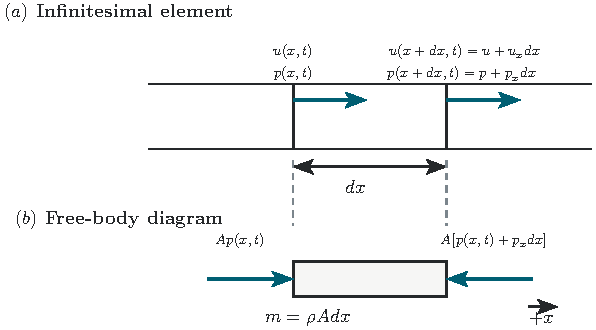
\includegraphics[width=0.86\linewidth]{figures/generated/solutions/B1-element-fbd.pdf}
\caption{Infinitesimal fluid element and its free-body diagram. The upper panel shows the pressure disturbance and axial displacement at each face. The lower panel shows the pressure forces acting on the isolated element.}
\end{figure}

\textbf{4. Newton's law of motion.} The pressure force on the left face is $A p(x,t)$ in the positive $x$ direction. The pressure force on the right face is $-A[p(x,t)+p_x(x,t)d x]$. Thus the net force is

\[
F_x=A p-A(p+p_xd x)=-A p_xd x.
\]

The element mass is $m=\rho A d x$, and its axial acceleration is $u_{tt}$. Newton's law gives

\[
-A p_xd x=(\rho A d x)u_{tt}.
\]

After canceling $A d x$, the pressure--acceleration relation is

\[
\boxed{p_x=-\rho u_{tt}}\qquad\text{(B.1.4)}
\]

The sign follows directly from the fact that pressure decreases in the direction of positive acceleration.

\textbf{5. Fluid elasticity.} The element volume is $V=A d x$. Its first-order volume change is

\[
\Delta V=A\bigl[u(x+d x,t)-u(x,t)\bigr]=A u_xd x.
\]

The fluid-elasticity relation is $\Delta P=-K\Delta V/V$. The equilibrium pressure is constant, so $\Delta P=p$. Therefore,

\[
p=-K\frac{A u_xd x}{A d x},
\qquad
\boxed{p(x,t)=-K u_x(x,t)}\qquad\text{(B.1.5)}
\]

Compression has $u_x<0$, which produces a positive pressure disturbance, consistent with the sign convention.

\textbf{6. Relationship between spatial and temporal derivatives.} Differentiating the elasticity relation with respect to $x$ gives $p_x=-K u_{xx}$. Equating this result to the Newton-law relation from item 4 gives

\[
-K u_{xx}=-\rho u_{tt},
\qquad
\boxed{K u_{xx}=\rho u_{tt}}\qquad\text{(B.1.6)}
\]

\textbf{7. Wavespeed.} Define the fluid wavespeed, also called the sound speed, by

\[
\boxed{c=\sqrt{\frac{K}{\rho}}}
\qquad\Longleftrightarrow\qquad
\boxed{c^2=\frac{K}{\rho}}\qquad\text{(B.1.7)}
\]

\textbf{8. Wave equation.} Dividing the relation from item 6 by $\rho$ and substituting $K/\rho=c^2$ yields the one-dimensional wave equation in the fluid,

\[
\boxed{u_{tt}=c^2u_{xx}}
\qquad\text{or equivalently}\qquad
\boxed{u_{xx}-\frac{1}{c^2}u_{tt}=0}\qquad\text{(B.1.8)}
\]

This equation describes small axial disturbances in the uniform inviscid fluid under the stated rigid-tube assumptions.
